\chapter{SCION/SCIONLab}
\section{SCION}
\acs{SCION} is a new internet architecture invented by Prof. Adrian Perrig and his fellow researchers. It's goal is to deliver scalability, control and isolation on next-generation networks. \acs{SCION} differentiates between a control plane and a data plane, which are completely separated from each other to increase robustness. Failures in the control plane therefore don't immediately affect the availability of the data plane and vice versa.

\subsection{Control Plane}
Since \acs{SCION} is an internet architecture it is designed to replace both \acs{IP} and \acs{BGP} and therefore fundamentally redesign the internet on \ac{OSI}-Layer 3 (Network Layer) and 4 (Transport Layer). Like the traditional internet, \acs{SCION} is organized in \aclp{AS}. But unlike the traditional internet, \acs{SCION} organizes multiple \acsp{AS} in so called \aclp{ISD}. Per \ac{ISD}, \acsp{AS} have the same \acl{TRC}.

\subsubsection{Path Construction}
Path construction in \acs{SCION} happens in two phases, path exploration and path registration. In the path exploration phase the core-\acsp{AS} send out \acp{PCB}. The \acsp{AS} can then decide to whom they want to forward the \acs{PCB}. Each \acs{AS} can then decide over which paths they want to be reached and register these paths in the path servers of the core-\acsp{AS}. These processes happen both within an \acs{ISD} as well as across \acsp{ISD}. The final path is then constructed out of three partial paths, an up-path, a down-path and a core path. How this final path is constructed is up to the \acs{AS} itself, which gives it control over the path a certain package takes to reach it's destination. For further details I recommend reading chapter 7 of \textit{SCION: A Secure Internet Architecture} \cite{perrig2017scion}

\subsection{Data Plane}
%TODO Check if lookup process is correct...
The data plane consists mainly of path combination and data forwarding. Each \acs{AS} possesses multiple up-paths. The down-paths are registered in the path servers of the core-\acsp{AS} of the destination's \acs{ISD} and can be requested by the \acs{AS}. The core paths are stored in the path servers of the core-\acsp{AS}. Therefore to get the possible paths to reach a destination \acs{AS}, the source \acs{AS} chooses an up-path to reach one of its core-\acsp{AS} and requests the paths to one of the destination's core-\acsp{AS}. Then it contacts the destination's core-\acs{AS} to request the down-paths to the destination \acs{AS}. Out of these three path segments the source \acs{AS} can then construct the final path. By doing so it can also take short cuts over peering-links or if the destination \acs{AS} lies on the up-path then it doesn't even need to contact any core-\acs{AS}.
\\
More details on how paths can be combined can be found in chapter 8 of the \acs{SCION}-book \cite{perrig2017scion}

\subsection{Joining a SCION Network}
For an \acs{AS} to join a \acs{SCION} network is quite easy. All the \acs{AS} has to do is setting up at least one path server, one beacon server, one certificate server and one \acs{SCION} border router. Then it buys connectivity from an AS that is already in the \acs{ISD} that the \acs{AS} wants to join as well. By joining the \acs{ISD} the \acs{AS} accepts the \acs{TRC} configured for this \acs{ISD}.

\subsection{Topology}
%TODO find a good figure to describe a typical SCION topology

\section{SCIONLab}
\acs{SCIONLab} is the distributed testbed for \acs{SCION}. Most of the network is managed by the Network Security Group of \acs{ETH} Zurich. The \acsp{AS} that are not managed by \acs{ETH} Zurich are called user-\acsp{AS}. Each of them is typically attached to one of the few \aclp{AP} that are part of the network infrastructure managed by \acs{ETH}. The \acsp{AP} are the only \acsp{AS} that allow direct connections to user-\acsp{AS}.
\\
The \acs{SCIONLab} network consists of multiple \acsp{ISD}, most of which are grouping together \acsp{AS} based on their geographic location or membership of a political union. However, one \acs{ISD} has the purpose of building a backbone for the entire \acs{SCIONLab} network. It is heavily interconnected and is hosted on \aclp{AWS}.

\subsection{SCIONLab as an Overlay Network}
%TODO check if it is always Ubuntu-16.04
Each \acs{SCIONLab}-\acs{AS} is based on a Ubuntu-16.04 machine. Either it is a \acl{VM} or a dedicated \acs{SCION} system. Each \acs{SCIONLab}-\acs{AS} has to at least have the following services available: 
\\
\begin{enumerate}
\item A \acl{BS} that sends and receives the \acsp{PCB}
\item A \acl{PS} that stores the path segments and disseminates them to the customers.
\item A \acl{CS} that holds the certificates which are used to validate the paths.
\item A \acl{BR} that routes (on a \acs{SCION}-level) the traffic leaving the \acs{AS}.
\end{enumerate}

As shown in figure \ref{SCIONLab-AS} the \acl{BR} is also responsible for wrapping the \acs{SCION}-traffic into \acs{IP}-traffic. This is simply done by setting up an \acs{IP}-connection to the corresponding \acl{AP} and then send the \acs{SCION} packets over that connection. It is important to note that the \acl{BR} doesn't do any routing on an \acs{IP}-level.

\begin{figure}[h]
	\centering
	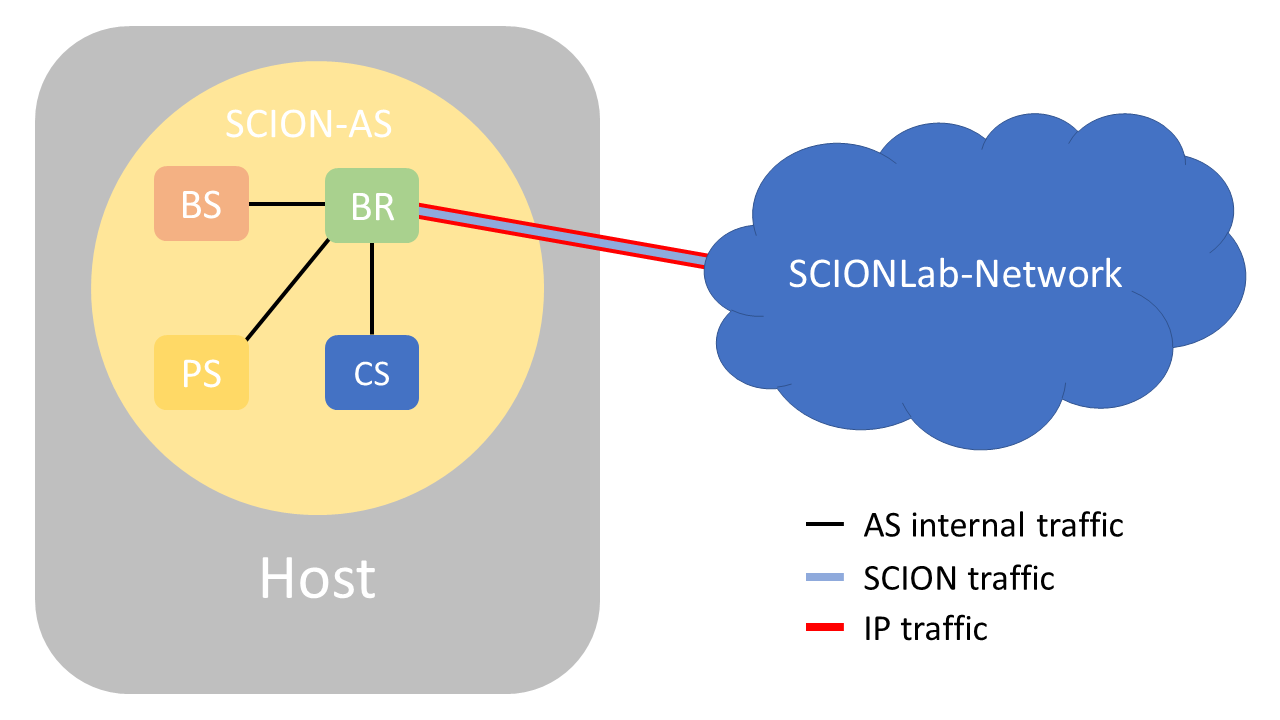
\includegraphics[width=\textwidth]{img/SCIONLab-AS.png}
	\caption{Schematic representation of a minimal SCIONLab-AS set-up}
	\label{SCIONLab-AS}
\end{figure}

\subsection{SCIONLab AS}
There are two main ways to set up a \acs{SCIONLab}-\acs{AS}. The most common one is to set it up in a \acs{VM}. The other option is to set it up on a dedicated \acs{SCION} system. Either way, you can do that by creating an account on \href{https://www.scionlab.org}{scionlab.org} and use the web interface to configure your \acs{AS} to your needs. This web portal is called \acs{SCIONLab} Coordination Service. After you configured your \acs{AS}, you can download the files that are used to either set up the \acs{VM} or the dedicated \acs{SCION} system. The \acl{AP} needs some time to receive the new configuration files to set up the connection to the user-\acs{AS}. When the \acs{AP} is ready, you will receive an e-mail that informs you about it. As visible in figure \ref{SCIONLab Coordination Service} the current version of the \acs{SCIONLab} Coordination Service doesn't allow you to configure any bandwidth limits.

\begin{figure}[h]
	\centering
	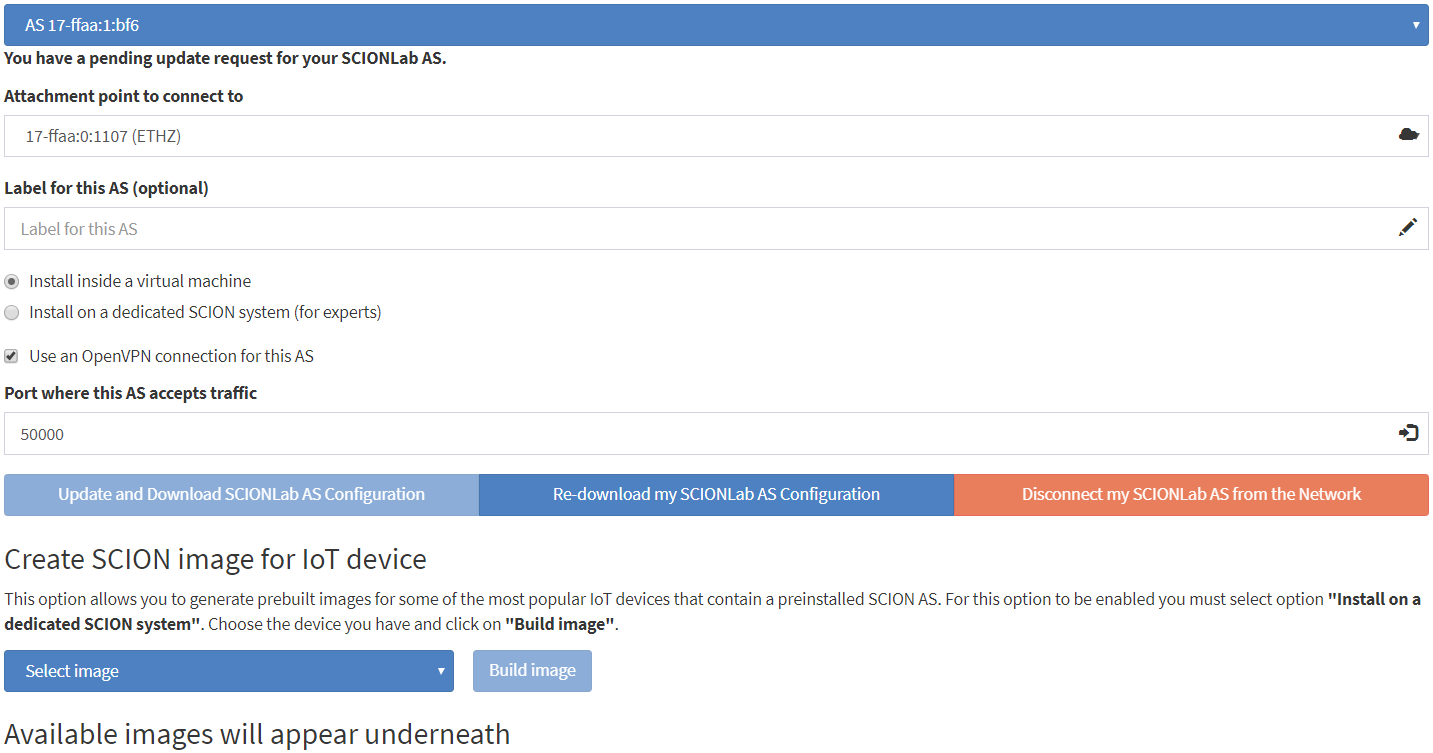
\includegraphics[width=\textwidth]{img/SCIONLab_Coordination_Service.png}
	\caption{Web Interface of the SCIONLab Coordination Service }
	\label{SCIONLab Coordination Service}
\end{figure}

\subsection{Topology}
%TODO find a good way to explain a typical SCIONLab topology
